\chapter{基于GPDD的电路简化原理}
\label{chap:gpddtheory}

上一章介绍了电路模型对电路设计的重要性,可见电路低阶模型本身的提出也应有一定方法可以指导其生成。
只有在拥有可靠的模拟集成电路低阶模型的情况下,电路设计工程师才有可能对电路做出进一步的理论分析,从而指导进一步的设计。
课件电路模型的生成需要电路拓扑的支持。
所以电路元件的拓扑结构对于分析本身有非常重要的作用。
本章对一些GPDD理论进行了补充,来建立GPDD结构和电路拓扑之间的关系。
并给出多端口电路的构造方法以及敏感度分析方法,以方便对多端口电路的分析及电路的优化。

\section{GPDD中的二元操作}

GPDD中有两种操作,分为将电路的元件值置为零,和将电路的元件值置为无穷大。
我们发现电路的元件的极限取值可以代表新的简化的电路拓扑结构。
这正可以成为我们对电路简化的基石。
当我们考虑需要将一个电路中的元件删去时,即可认为是电路这个元件选取了极限的取值导致。
当然一个电路元件删去过程中,往往存在两个电路元件删去方式:短路和断路。

\begin{figure}[!htp]
	\centering
	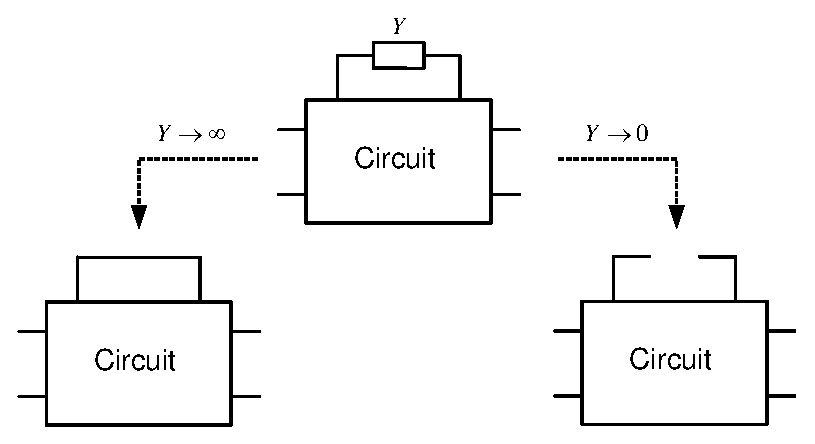
\includegraphics[width=0.7\textwidth]{chap2/LimitTopo.eps}
	\bicaption[fig:limittopo]{导纳在极限取值情况下的拓扑结构改变}{导纳在极限取值情况下的拓扑结构改变}{Fig}{Topological adjustment of impedance whose value changes to limit value}
\end{figure}

如图\ref{fig:limittopo}所示,假设在一个电路中有一处导纳值为$Y$的阻抗。
现在我们用两个极限的值$\infty$和$0$去替代这个导纳值$Y$。
可以看到当,导纳值$Y$趋向于无穷大时,由于此时其相应的阻抗$Z$为零,所以此时这个阻抗变为短路的电路结构;
然而当导纳值$Y$趋向于零时,由于此时其阻抗值$Z$为无穷大,这种情况下电路结构变为阻抗两端的两个节点变为了断路的状态。
可以看到,这样我们就可以用电路元件的极限取值来替代线性阻抗元件(R/L/C)的拓扑变化。

然而,在小信号电路中,我们知道不仅存在线性阻抗元件(R/L/C),另外还有四种受控信号源,分别为:电压控制电压源(VCVS),电流控制电流源(CCCS),电压控制电流源(VCCS),电流控制电压源(CCVS)。
我们发现在以上两种极限取值仍然适用于这四种受控源,特别是在取无穷大情况下,它们都会成为一种称为Nullor的电路元件,如图\ref{fig:nullor}。

\begin{figure}[!htp]
	\centering
	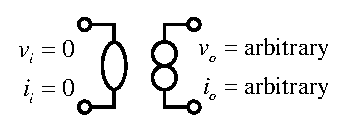
\includegraphics[width=0.35\textwidth]{chap2/SymbolNullor.eps}
	\bicaption[fig:nullor]{Nullor元件符号}{Nullor元件符号}{Fig}{Nullor symbol}
\end{figure}

可以看到,Nullor元件假设其输入端的输入电流和电压均为0,有着任意大小的输出能力。
Nullor这种元件与传统的模拟电路学习中接入负反馈中的理想运算放大器的虚短虚断的性质是一致。
但由于Nullor本身往往可以与电路中别的元件合并,并且不会出现在电路最后的模型中,这一点会在本章中节\ref{subsubsec:simp:res:cir:fd}中看到。

\begin{table}[!htbp]
	\bicaption[tab:symbollimit]{电路元件极限取值的拓扑结构}{电路元件极限取值的拓扑结构}{Table}{Circuit element topology whose value is infinity or zero}
	\centering
	\begin{tabular}{c|c|c}
		\hline
		\multirow{2}{*}{Symbol} & \multicolumn{2}{c}{Value}\\
		\cline{2-3} 
		& $\infty$ & $0$\\
		\hline
		\parbox[c]{0.11\textwidth}{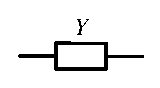
\includegraphics[width=0.11\textwidth]{chap2/Impedance.eps}} & 
		\parbox[c]{0.11\textwidth}{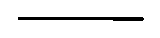
\includegraphics[width=0.11\textwidth]{chap2/Impedance-Short.eps}} & 
		\parbox[c]{0.11\textwidth}{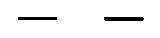
\includegraphics[width=0.11\textwidth]{chap2/Impedance-Open.eps}} \\
		\hline
		\parbox[c]{0.2\textwidth}{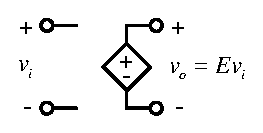
\includegraphics[width=0.2\textwidth]{chap2/VCVS.eps}} & 
		\parbox[c]{0.11\textwidth}{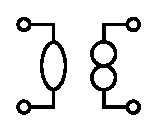
\includegraphics[width=0.11\textwidth]{chap2/Nullor.eps}} & 
		\parbox[c]{0.11\textwidth}{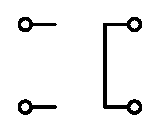
\includegraphics[width=0.11\textwidth]{chap2/VCVS-Open.eps}} \\
		\hline
		\parbox[c]{0.2\textwidth}{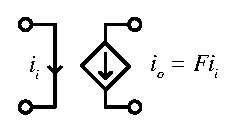
\includegraphics[width=0.2\textwidth]{chap2/CCCS.eps}} & 
		\parbox[c]{0.11\textwidth}{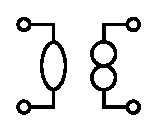
\includegraphics[width=0.11\textwidth]{chap2/Nullor.eps}} & 
		\parbox[c]{0.11\textwidth}{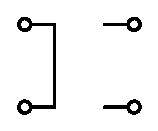
\includegraphics[width=0.11\textwidth]{chap2/CCCS-Open.eps}} \\
		\hline
		\parbox[c]{0.2\textwidth}{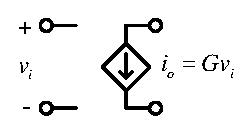
\includegraphics[width=0.2\textwidth]{chap2/VCCS.eps}} & 
		\parbox[c]{0.11\textwidth}{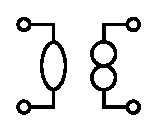
\includegraphics[width=0.11\textwidth]{chap2/Nullor.eps}} & 
		\parbox[c]{0.11\textwidth}{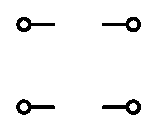
\includegraphics[width=0.11\textwidth]{chap2/VCCS-Open.eps}} \\
		\hline
		\parbox[c]{0.2\textwidth}{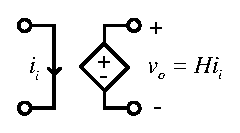
\includegraphics[width=0.2\textwidth]{chap2/CCVS.eps}} & 
		\parbox[c]{0.11\textwidth}{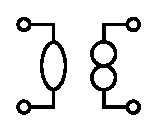
\includegraphics[width=0.11\textwidth]{chap2/Nullor.eps}} & 
		\parbox[c]{0.11\textwidth}{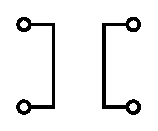
\includegraphics[width=0.11\textwidth]{chap2/CCVS-Open.eps}} \\
		\hline
	\end{tabular}
\end{table}

为了说明受控源取极限值情况下电路拓扑结构的变化,这里仅以VCVS为例进行说明。
所有小信号分析中用到的阻抗和四种受控源的拓扑变化可以参考表\ref{tab:symbollimit}。
我们知道VCVS的输入输出电压关系如下式所示:

\begin{equation}
v_o = E v_i
\end{equation}

这里,$v_i$和$v_o$分别为VCVS的输入输出电压,$E$则为VCVS的放大倍数。
首先我们考虑$E$取无穷大的情况,为了电路仍然能正常工作,我们知道输出电压$v_o$应为有限值,而其中$E$为无穷大,那么根据基本微积分的知识,我们知道此等式中的输入电压$v_i$为零。
另外由于VCVS的输入端测量电压,所以本来就限定输入的电流$i_i$为零,所以其形成了Nullor的虚短虚断的性质。
另外当$E$的取值为零时,根据VCVS本身的关系,即可得出输出端电压为零,所以输出端两端电压一致,即此端口可用一根导线连接起来,加之本为断路连接的输入端,故VCVS可约减为表\ref{tab:symbollimit}中的结构。

\section{GPDD与电路拓扑结构的对应关系}

上一小节已经将GPDD的二元操作与电路的拓扑结构变化建立起了联系,而此时电路元件的极限求值成为了新的问题。
由于在整个算法过程中,需要多次计算不同拓扑结构下电路性能表现,这要求了高效的计算方法的支持。
然而GPDD结构本身蕴含了对电路拓扑结构,可以轻松方便地在其中对不同的电路拓扑结构求值,这支持了下一节所介绍的简化算法。

\begin{figure}[!htp]
	\centering
	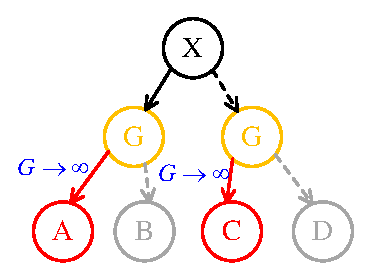
\includegraphics[width=0.35\textwidth]{chap2/GPDDTopo.eps}
	\bicaption[fig:GPDDTopo]{符号极限取值情况下GPDD的计算方法}{符号极限取值情况下GPDD的计算方法}{Fig}{Calculation rule for GPDD under limit value}
\end{figure}

我们知道根据电路基本原理,并且结合GPDD的计算规则,针对类似图\ref{fig:GPDDTopo}这样的GPDD结构,我们可以求得类似下式的电路传输函数表达式(为了说明的方便,这里忽略了GPDD中连接节点的边上的符号):

\begin{equation}
H \left( s \right) = \frac{{{f_A}\left( A \right)G + {f_B}\left( B \right)}}{{{f_C}\left( C \right)G + {f_D}\left( D \right)}}
\end{equation}

考虑目前我们需要对电路中的元件$G$求取极限值,并计算新的符号化传输函数公式。
这里假设元件$G$位于GPDD符号表中的第一层,这里层数不影响极限取值的计算,只是为方便说明特意假设。
我们可以得到在$G$元件取无穷大情况下,电路的新传输函数为:

\begin{equation}
\label{eq:simpGPDD}
\mathop {\lim }\limits_{G \to \infty } H \left( s \right) = \frac{{f_A}\left( A \right)}{{f_C}\left( C \right)}
\end{equation}

首先,十分显然地,可以看到取极限后首先原有的符号$G$从公式消失了,这也暗示了电路拓扑的简化,即$G$从电路中以短路的方式被删去了。
另外,可以发现,在式\ref{eq:simpGPDD}中所有的保留下的符号项均是在GPDD结构中以红色实线相连的红色节点$A$和$C$的值。
由于,我们知道,GPDD结构中实线相连的节点均采用乘法进行计算,故在求取极限的过程中,其相应的系数得到保留。
故当某一符号元件需取无穷大情况下的值时,在GPDD计算过程中,仅需计算GPDD对应符号所有节点左儿子的值即可,所有的右儿子忽略。
同样的,我们知道当对一个电路元件取值零时,GPDD计算中仅需考虑该元件所有节点右儿子的值即可,左儿子的值则忽略,而且算法设计简单,仅需直接用0带入符号值即可。
总结来说,GPDD中某个节点左儿子承担了该节点符号取值无穷大情况(阻抗短路,受控源Nullor)下的电路性能,而右儿子为该节点符号取值零情况(阻抗断路,受控源删去)下的电路性能,当符号本身有一定值时,则为两者的折衷。

当然需要注意的是,在求某一个符号为无穷大时,由于特殊的GPDD规模缩小的算法,类似Reduction、Zero-Suppression等算法\parencite{GShi-GPDD-2013,GShi-GPDD},可能存在有排序在$G$之上的符号直接与排序在$G$之下的符号节点相连的情况。
这种情况需特别注意,因为这种项中不包含$G$符号,故取极限值时,并非系数,也需忽略。
具体的GPDD中符号约减下的计算方法已在\parencite{HanbinHu-Thesis}有阐释,这里不再赘述。

下面通过一个例子展示电路拓扑结构变化对GPDD结构的影响,以直观了解这两者之间的关系。

\begin{exmp}
	RLC电路向RC电路简化过程中GPDD结构比较
	
	图\ref{fig:RLC}中展示了一个RLC串联的简易电路,与之前给出的图\ref{fig:RC_cir}相比较,这里多出了电感元件。
	可以看到如果这个电感$L$如果取值为零,那么其导纳$Y=\left(s L\right)^{-1}$,即导纳为无穷大情况,即可得到RC电路的电路图。
	
	\begin{figure}[!htp]
		\centering
		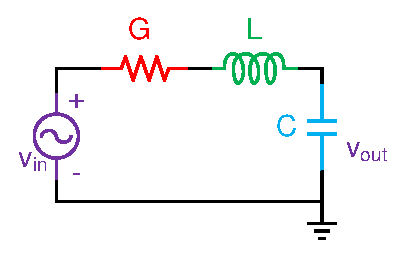
\includegraphics[width=0.4\textwidth]{chap2/RLC.eps}
		\bicaption[fig:RLC]{RLC电路示意图}{RLC电路示意图}{Fig}{RLC circuit example}
	\end{figure}
	
	此RLC电路对应的GPDD结构展示在图\ref{fig:RLCvsRC}中的左侧。这张图右侧是展示的RC电路对应的GPDD结构。
	可以看到通过两侧曲线包围起来的结构是一致的,而且均与电感符号$L$的左儿子相连,这与之前的论述是相符的。
	同时可以看到,由于RC的GPDD结构蕴含在RLC的GPDD结构中,故可以直接在RLC的GPDD结构上对RC电路的GPDD进行求值。
	这表示了GPDD拥有在同一个BDD数据结构中求解多种不同电路拓扑的能力,这大大方便了符号简化电路自动生成算法的设计。
	这种能在同一个符号化结构中表达不同拓扑结构电路的能力是别的符号化方法不具备的,也是GPDD相比其他的符号化方法一大优势所在。
	
	\begin{figure}[!htp]
		\centering
		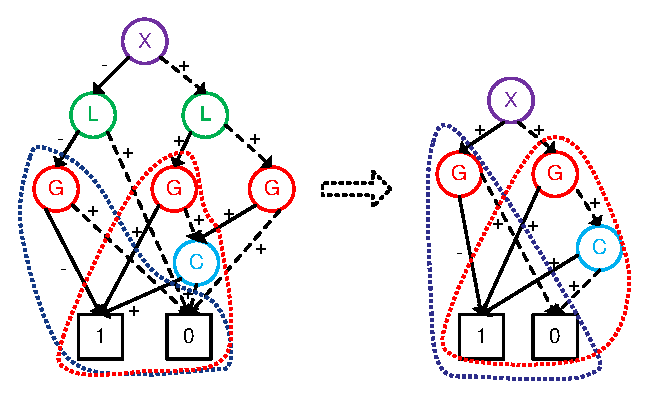
\includegraphics[width=0.7\textwidth]{chap2/RLCvsRC.eps}
		\bicaption[fig:RLCvsRC]{符号极限取值情况下GPDD结构示例}{符号极限取值情况下GPDD结构示例}{Fig}{GPDD structure example under limit value}
	\end{figure}
	
\end{exmp}

GPDD对低阶模型生成过程中的求解优势在于在一次符号表达构造的情况下,可以在多次同一个结构中求得对应与不同简化模型的电路传输函数。
符号化构造往往大量计算时间花费在符号化表达式的构造上,而其求值往往是高效的稳定的。
故可以如将构造的时间平摊在之后的多次求值上,仍然得到了许多计算上的便利。
同时,如采用传统的数值化求解器,需要对电路矩阵做行列合并等操作,操作复杂。

\section{多端口构造原理}
\label{sec:mp}

传统的多端口GPDD构造方法会构造一个多根的GPDD结构,并在每个根中生成对应的图对,用于接下来的展开过程\parencite{GShi-GPDD-2013}。
本文则证明了当电路满足一定条件情况下,电路的GPDD构造可以使用一个单根的结构来替代,而不需要多根的展开过程。
这么做的好处主要是可以复用原有的GPDD展开代码,避免了引入新的程序错误,加快了开发效率,减少花费在程序实现上的工作量。

\begin{figure}[!htp]
	\centering
	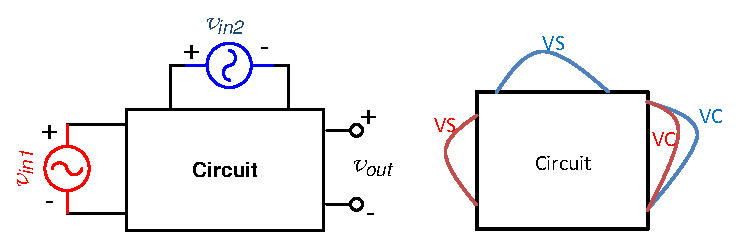
\includegraphics[width=0.8\textwidth]{chap4/MultiPort.eps}
	\bicaption[fig:mp]{多端口电路示意}{多端口电路示意}{Fig}{Multi-Port circuit example}
\end{figure}

假设我们考虑如图\ref{fig:mp}左侧所示的电路结构。
这里电路总共有两个输入端口,而且两个输入端口共享同一个电路输出端口。
将这样的电路结构画成如图\ref{fig:mp}右侧的图,可以看到在输出端口有两条并联的VC边。
由于GPDD算法是对电路中生成树对的枚举过程,所以如果两条VC同时出现在最终的生成树对中,则会形成环路。
所以如图\ref{fig:mpgpdd},必然不会出现两个输入对以实线边相连的情况。

\begin{figure}[!htp]
	\centering
	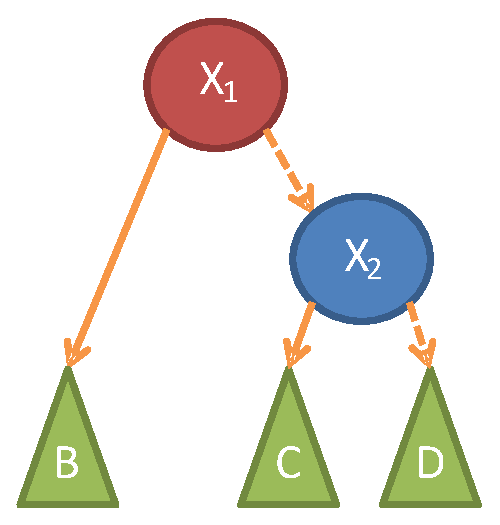
\includegraphics[width=0.3\textwidth]{chap4/MultiPortGPDD.eps}
	\bicaption[fig:mpgpdd]{多端口电路的GPDD结构}{多端口电路的GPDD结构}{Fig}{GPDD structure for multi-port circuit example}
\end{figure}

这里我们用符号$X_1$和$X_2$代表两组输入输出关系。如需要对电路传输函数进行计算,根据本前面内容中介绍的元件拓扑结构与GPDD之间的关系,我们可以发现某个传输函数即是在另一个输入输出对符号置零情况下得到的结果。区别于之前章节的记号,这里使用比较简单易写的$f\left( N \right)$来作为节点$N$的GPDD计算结果。所以可以根据下两式对电路的传输函数进行计算:

\begin{eqnarray}
{H_1}\left( s \right) = \frac{{{v_{out}}}}
{{{v_{in1}}}} = \frac{1}
{{{X_1}}} = \frac{{f\left( B \right)}}
{{f\left( D \right)}} \hfill \\
{H_2}\left( s \right) = \frac{{{v_{out}}}}
{{{v_{in2}}}} = \frac{1}
{{{X_2}}} = \frac{{f\left( C \right)}}
{{f\left( D \right)}} \hfill 
\end{eqnarray}

另外可以看到电路传输函数共享同一个分母,这与基本电路两端口的性质是一致的。
只要在满足如下定理的情况下,这种情况在推广到更多的端口与更大的电路规模仍然成立。

\begin{thm}\label{thm:mpcon}
	在满足以下条件之一的情况下,GPDD可以用单根构造的方式构造多端口电路,且不会出现多个输入输出端口符号的交叉项:
	\begin{enumerate}[label=\emph{\alph*})]
		\item 所有端口的输出端均在同一端口测量同种信号(电流或电压)。
		\item 所有端口的输入端均在同一端口施加同种信号(电流或电压)。
	\end{enumerate}
\end{thm}

这里使用生成树对枚举的方式对定理的正确给出说明。我们只对输出端可能出现的$VC$边和$CC$边进行说明,输入端的$VS$和$CS$可以类比得到。

首先来考虑VC边,我们知道,对同一个端口的电压进行测量,那么相应的所有的$VC$边必然并联。
那么很明显如果有多个$VC$被包含的情况下,必然形成环,不会出现树的结构,故生成的GPDD中必然不含有有多个输入输出端口符号的符号化项。
其次我们考虑CC边,对同一个端口的电流进行测量,那么相应的所有的$CC$边必然串联。
根据GPDD理论\parencite{GShi-GPDD},如需符号项需包含有CC边的符号,那么在生成树对中的左树中CC边并不会包含在最终的树中。
由于,$CC$边串联,故如有两个或以上输入输出符号被包含在符号项中时,必然造成图中出现了分离的图,而分离的图无法生成树结构。
这样的话我们就可以得到定理\ref{thm:mpcon}的条件a,条件b可以用类似的方法说明。

\section{符号化敏感度分析方法}

GPDD理论中关于电路的敏感度分析将大大有助于模拟电路工程师加深对电路设计的理解,帮助电路工程师对电路性能优化提供更多的具有洞察力的信息\parencite{MengXiaoxuan-Sens-2009,WengBinbin-Sens-2011,ChenJiajun-Sens-2012}。

这里对符号化敏感度分析做一定回顾,并给出考虑CMRR和PSRR特殊情况下的计算规则。敏感度定义如下:

\begin{equation}
Sens\left( {H\left( s \right),p} \right) = \mathop {\lim }\limits_{\Delta p \to \infty } \left\{ {\frac{{\frac{{\Delta H\left( s \right)}}{{H\left( s \right)}}}}{{\frac{{\Delta p}}{p}}}} \right\} = \frac{p}{{H\left( s \right)}}\frac{{\partial H\left( s \right)}}{{\partial p}}
\end{equation}

敏感度反应了电路传输函数$H\left(s\right)$的变化对参数$p$的变化的所产生的影响。
可以想象若敏感度绝对值很高,则$p$的变化会引起较大的数$H\left(s\right)$的改变。若我们选择各个MOS晶体管的宽$W$为$p$,那么就可以求得电路元件尺寸与电路性能直接关系,则可以得到如下公式。

\begin{equation}\label{eq:DCSens}
Sens\left( {H\left( s \right),{W_i}} \right) = \frac{{{W_i}}}{{H\left( s \right)}} \sum\limits_{j} \sum\limits_{p} {\frac{{\partial H\left( s \right)}}{{\partial {g_{j,p}}}}\frac{{\partial {g_{j,p}}}}{{\partial {W_i}}}}
\end{equation}

其中$W_i$为电路中$i$号MOS管的宽,而$g_{ij}$则为i号MOS管的第j个小信号参数,如:$g_m$,$g_{ds}$,$g_{mb}$,$c_{gs}$等。
可以看到,若我们忽略别的晶体管对$i$号晶体管小信号参数的影响,则上述公式最右侧的式子中H(s)可以由GPDD进行计算,而第二个偏导数可以由器件模型以及DC偏置点决定。
我们通过一个例子来进一步解释式\ref{eq:DCSens}的意义。

\begin{exmp}
	运放中的敏感度公式意义
	
	\begin{figure}[!htp]
		\centering
		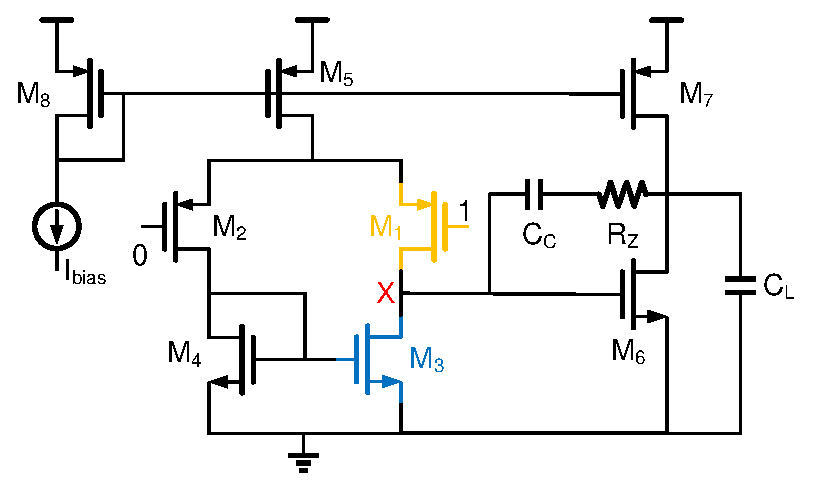
\includegraphics[width=0.7\textwidth]{chap4/TSExample.eps}
		\bicaption[fig:tsexample]{用于敏感度说明的两级运放电路}{用于敏感度说明的两级运放电路}{Fig}{Two-stage opamp for sensitivity explanation}
	\end{figure}
	
	考虑图\ref{fig:tsexample}中的运放电路,如果我们需要对这里的$M_1$管的宽$W_1$进行敏感度分析。
	根据式\ref{eq:DCSens}中所示,可以得到如下的推导:
	
	\begin{align}
		Sens\left( {H\left( s \right),{W_1}} \right) &= \frac{{{W_1}}}
		{{H\left( s \right)}}\frac{{\partial H\left( s \right)}}
		{{\partial {W_1}}} \nonumber \\ 
		&= \frac{{{W_1}}}
		{{H\left( s \right)}}\left( {\sum\limits_p {\frac{{\partial H\left( s \right)}}
				{{\partial {g_{1,p}}}}\frac{{\partial {g_{1,p}}}}
				{{\partial {W_1}}}}  + \sum\limits_{j \ne 1,p} {\frac{{\partial H\left( s \right)}}
				{{\partial {g_{j,p}}}}\frac{{\partial {g_{j,p}}}}
				{{\partial {W_1}}}} } \right) \nonumber \\ 
		&= \frac{{{W_1}}}
		{{H\left( s \right)}}\left( {\frac{{\partial H\left( s \right)}}
			{{\partial {\textcolor{orange}{g_{m1}}}}}\frac{{\partial {\textcolor{orange}{g_{m1}}}}}
			{{\partial {W_1}}} +  \cdots  + \frac{{\partial H\left( s \right)}}
			{{\partial {\textcolor{blue}{g_{ds3}}}}}\frac{{\partial {\textcolor{blue}{g_{ds3}}}}}
			{{\partial {\textcolor{red}{V_X}}}}\frac{{\partial {\textcolor{red}{V_X}}}}
			{{\partial {W_1}}} +  \cdots } \right)
	\end{align}
	
	可以看到在最后一步中展开的两项中,其中第一项仅与$M_1$管的参数有关,而第二项还与$M_3$管有关。
	造成这种现象的原因主要在于当改变$W_1$的时候,必然会对$X$节点的电压造成影响,故会影响$M_3$管偏置情况,故此时可与$M_3$管中的小信号参数相关。
	
\end{exmp}

关于式\ref{eq:DCSens}第一项偏导数的计算,其实十分类似我们选取元件取值为无穷大是的计算过程,首先我们假设$H\left(s\right)$的公式如下式所示:

\begin{equation}
H\left( s \right) = \frac{{N\left( s \right)}}{{D\left( s \right)}} = \frac{{{N_1}\left( s \right)Y + {N_2}\left( s \right)}}{{{D_1}\left( s \right)Y + {D_2}\left( s \right)}}
\end{equation}

我们知道线性电路的传输函数一定是一个有理多项分式。
故分子$N\left(s\right)$和分母$D\left(s\right)$均为乘积项之和(Sum of Products,SOP)的形式,且显然分别为GPDD根节点的左右子结构。
$Y$是电路中某个元件的导纳值或者受控源的系数。
显然,我们可以将$N\left(s\right)$和$D\left(s\right)$分解为不包含$Y$这一项的$N_1\left(s\right)$、$N_2\left(s\right)$、$D_1\left(s\right)$和$D_2\left(s\right)$四个式子。
可以注意到由于GPDD结构节点求值的方法,每个节点总是乘以左边的节点的值并加上右边节点的值。
故可以想到$N_1\left(s\right)$是GPDD根节点左侧子结构中忽略所有Y节点的右边连接关系得到的结果,以此类推,可以得到$N_2\left(s\right)$、$D_1\left(s\right)$和$D_2\left(s\right)$相应在GPDD中对应的结构。
对于求取偏导数,我们有

\begin{equation}
\frac{{\partial H\left( s \right)}}
{{\partial Y}} = \frac{{\frac{{\partial N\left( s \right)}}
		{{\partial Y}}D\left( s \right) - N\left( s \right)\frac{{\partial D\left( s \right)}}
		{{\partial Y}}}}
{{{D^2}\left( s \right)}} = \frac{{{N_1}\left( s \right)D\left( s \right) - N\left( s \right){D_1}\left( s \right)}}
{{{D^2}\left( s \right)}}
\end{equation}

上式表示传输函数针对某个电路元件Y的偏导数与$N\left(s\right)$,$D\left(s\right)$,$N_1\left(s\right)$和$D_1\left(s\right)$有关。
可以注意到仅有与$Y$相乘的项得到了保留,相对应的在GPDD中,即仅有与$Y$节点的左边节点才计入计算,右边节点则忽略,这与求取元件无穷大取值情况下的GPDD计算是一致的。
同样的,同时需要注意到由于GPDD的共享性质,有些从根节点到1结点的路径不会经过Y节点,这种项也不能计入其中。

\section{本章小结}

本章给出了一系列有关GPDD电路简化的理论与敏感度分析的方法,并通过多个电路实例向读者介绍这些理论的具体意义。
这些理论建立了电路元件取值与电路拓扑结构之间的关系,为下一步的电路低阶模型的生成打下了坚实的理论基础。
多端口构造理论在分析含有多端口的电路情况下,可以有大量的应用,如同时分析CMRR、PSRR等。
敏感度分析往往可以用于电路的元件尺寸的优化改进等方面,方便了电路的调整。